\documentclass{article}

\usepackage{amsmath}
\usepackage{tikz}
\usetikzlibrary{arrows}

\begin{document}

\section{Homogenous Transformation}

Two frames $o_0 x_0 y_0 z_0$ and $o_1 x_1 y_1 z_1$ are related by
	the homogenous transformation, which sends frame 0 to frame 1:

\begin{align}
H & = \left[ \begin{matrix}
	0 & -1 & 0 & 1 \\
	1 & 0  & 0 & -1 \\
	0 & 0 & 1 & 0 \\
	0 & 0 & 0 & 1 
\end{matrix} \right] \label{eq:def-of-H}
\end{align}

A particle has velocity $v_1(t) = \left[ 3, 1, 0 \right]^T$ relative
	to the frame $o_1 x_1 y_1 z_1$.
Since the velocity and the frame are both constant, to find the velocity
	in frame zero, it suffices to express the vector $v_1$ in frame 0.
The inverse transformation is:

\begin{align*}
H^{-1} & = \left[ \begin{matrix}
	0 & 1 & 0 & -1 \\
	-1 & 0  & 0 & 1 \\
	0 & 0 & 1 & 0 \\
	0 & 0 & 0 & 1 
\end{matrix} \right]
\end{align*}

Since $v_1$ is a vector, the rotation is all that we need to consider.
Therefore, $v_0$ is:

\begin{align*}
\left[ \begin{matrix}
	0 & 1 & 0 \\
	-1 & 0 & 0 \\
	0 & 0 & 1 \end{matrix} \right]
\left[ \begin{matrix}
	3 \\
	1 \\
	0 \end{matrix} \right]
& =
\left[ \begin{matrix}
	1 \\
	-3 \\
	0 \end{matrix} \right]
\end{align*}

\section{Jacobian for 3-link Elbow Manipulator}

Compute the jacobian $J_{11}$ for the 3-link elbow manipulator of Example 4.9
	and show that it agrees with Equation (4.98).

From Eq. 4.58, if there are only revolute joints on a manipulator,
	
\begin{align}
J_{v_i} = z_{i-1} \times \left( o_n - o_{i-1} \right) \label{eq:def-of-Jvi}
\end{align}

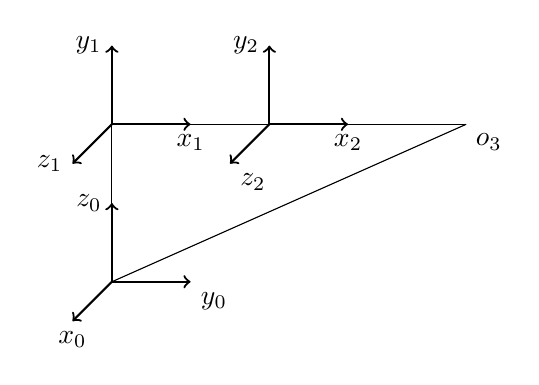
\begin{tikzpicture}
\coordinate (origin) at (0,0);
\draw[->, thick] (origin) to (-0.5,-0.5) node[below] (x0) {$x_0$};
\draw[->, thick] (origin) to (1,0) node[below right] (y0) {$y_0$};
\draw[->, thick] (origin) to (0,1) node[left] (z0) {$z_0$};

\coordinate (o1) at (0,2);
\draw[-] (origin) to (o1);
\draw[->, thick] (o1) to (1,2) node[below] (x1) {$x_1$};
\draw[->, thick] (o1) to (0,3) node[left] (y1) {$y_1$};
\draw[->, thick] (o1) to (-0.5, 1.5) node[left] (z1) {$z_1$};

\coordinate (o2) at (2,2);
\draw[-] (o1) to (o2);
\draw[->, thick] (o2) to (3,2) node[below] (x2) {$x_2$};
\draw[->, thick] (o2) to (2,3) node[left] (y2) {$y_2$};
\draw[->, thick] (o2) to (1.5, 1.5) node[below right] (z2) {$z_2$};

\coordinate (o3) at (4.5,2);
\node[below right] (end) at (o3) {$o_3$};
\draw[-] (o2) to (o3);

\draw[-] (origin) to (o3);

\end{tikzpicture}

Show that the determinant agrees with Equation (4.99).

\end{document}
